\documentclass[12pt]{article}
\usepackage{blindtext}
\usepackage{lmodern}
\usepackage[utf8]{inputenc}
\usepackage[margin=0.7in]{geometry}

\usepackage{graphicx}
\graphicspath{ {./images/} }

\title{%
    COMP3702 - Artificial Intelligence \\
        Week 1 - Lecture Notes \\
        Module 0: Introduction}
        
\author{Anindya Sarup}

\date{7th August 2020}

\setcounter{secnumdepth}{0}

\setcounter{tocdepth}{5}

\begin{document}

\maketitle

\section*{Overview of Module 0}

What will be covered in Module 0:
\begin{enumerate}
    \item What is AI?
    \item History of Artificial Intelligence
    \begin{itemize}
        \item A very brief history of it
    \end{itemize}
    \item Intelligent Agents
    \item Goals of Artificial Intelligence
    \begin{itemize}
        \item Or what the purpose of developing intelligent agents is
    \end{itemize}
    \item Intelligent agents acting in an environment
    \item Dimensions of Complexity
    \begin{itemize}
        \item What are the dimensions of complexity of these agents at the stage of designing.
    \end{itemize}
\end{enumerate}

\newpage

\tableofcontents

\newpage

\section{What do you think AI is?}
The study and designs of mechanisms that...
\begin{itemize}
    \item think like humans? 
    \begin{itemize}
        \item Build something like a brain! But how does a human brain work?
        \item It is hard to build something like a brain, because we do not at a physical level know how a brain works, like spikes but we use back propagation which brain does not do.
        \item Thus, modelling a brain for building AI is becoming rather hard in practice. It's more the domain of something like cognitive or neuro-science.
        \item add image from lecture notes here
    \end{itemize}
    \item think rationally?
    \begin{itemize}
        \item Automated reasoning and logic are foundational topics in AI, that is, things that have been examined under the umbrella of AI for over 70 years.
        \begin{itemize}
            \item But is this a complete answer? As it is unclear if logic really captures the type of knowledge that people have or need help with.  
            \item Plus it's really hard to search through logical statements. The logical foundations of math are really solid but using that in an automated decision support system is not necessarily going to get you really far because it is difficult to search through logical statements.
            \item For example, if you have a ground set of logical statements with binary variables (similar to truth tables 0s \& 1s), then all the different ways you can combine these values grows exponentially with different combinations. Thus making it very difficult to setup very complex logical systems and then ascertain whether they are doing it what you expect them to do or helping you make decisions.
            \item Logic will be touched upon in Module 2.
        \end{itemize}
        \item Is there a need to constrain the working of AI to have the same mechanism like the brain or can we have it think like a brain?
        \item Thinking "rationally" has not been defined yet, but will be defined later on
    \end{itemize}
    \item act like humans?
    \begin{itemize}
        \item The Turing test: can a human tell if a computer is a computer?
        \item Setting the threshold to be whether a machine can be distinguished from a human is a novel goal.
        \item The Turing Test - Alan Turing (1950) 
        \begin{itemize}
            \item In the Turing test, the computer is asked questions by a human interrogator. 
            \item The interrogator asks questions to either a computer or a human. The questions are usually tricky, thus their correct answers are associated to being intelligent. Such questions are usually easy for a human to answer but are tricky for a machine to answer.
            \item Computer passes the test if the interrogator cannot tell whether the responses come from a human or a computer.
            \item The Turing test simplifies the question "is the machine intelligent" into "can the machine imitate a human?"
            \item Add image from lecture slides.
        \end{itemize}
        \item Lets stop and think: Do we really want computers to act like humans?
    \end{itemize}
    \item act rationally?
    \begin{itemize}
        \item Perhaps, what we really want are machines that \textbf{\emph{act rationally}}, that make better decisions for the sort of problems that they are very good at solving. This is known as \textbf{\emph{acting rationally}}
        \item Underpinning the idea of acting rationally is what is known as \textbf{\emph{Intelligent Agents}} (approach taken in R\&N and P\&M texts)
        \item That is, an Intelligent, rational, autonomous agent, a computational device or system that can make decisions on your behalf or control systems in the absence of a human or even provide advice on what it is you should be doing or what you might want to do in a given situation based on the way it reasons and learns about the world.
    \end{itemize}
    \item Not sure that this truly captures the variety of AI research going on right now, but it is a good place to start. 
    \item \emph{In this course, we are going to be building computational agents that act rationally in given environments and can learn from those environments.}
\end{itemize}

\subsection{So what really is AI?}
\begin{itemize}
    \item According to the Association for the Advancement of Artificial Intelligence (AAAI) offers this on its home page:\textbf{AI is "the scientific understanding of the mechanisms underlying thought and intelligent behavior and their embodiment in machines"}
    \item Poole and Mackworth say AI is \textbf{"the synthesis and analysis of computational agents that act intelligently."} This is in-sync with what their textbook on AI is about.
    \item According to our lecturer Archie: \textbf{"AI is the study and development of algorithms for solving problems that we typically associate with intelligence."} This leaves the interpretation of intelligence to be open.
\end{itemize}

\noindent In general, AI is a disperse collection of topics. In this course, we address core method and models used in AI research and practice, many of which have found a wide-spread use application and as building-blocks in more sophisticated AI systems. 
\emph{That's the high level mapping of AI to what we do in this course.}

\noindent All components of AI are not addressed in this course, specially topics like machine learning. Although, there is some usage of reinforcement learning and a little bit of neural networks.

\newpage
\section{(A very brief) History of Artificial Intelligence}

\emph{For more on the history and development of AI, read chapter 1 of R\&N or P\&M}

\begin{figure}[h!]
        \centering
        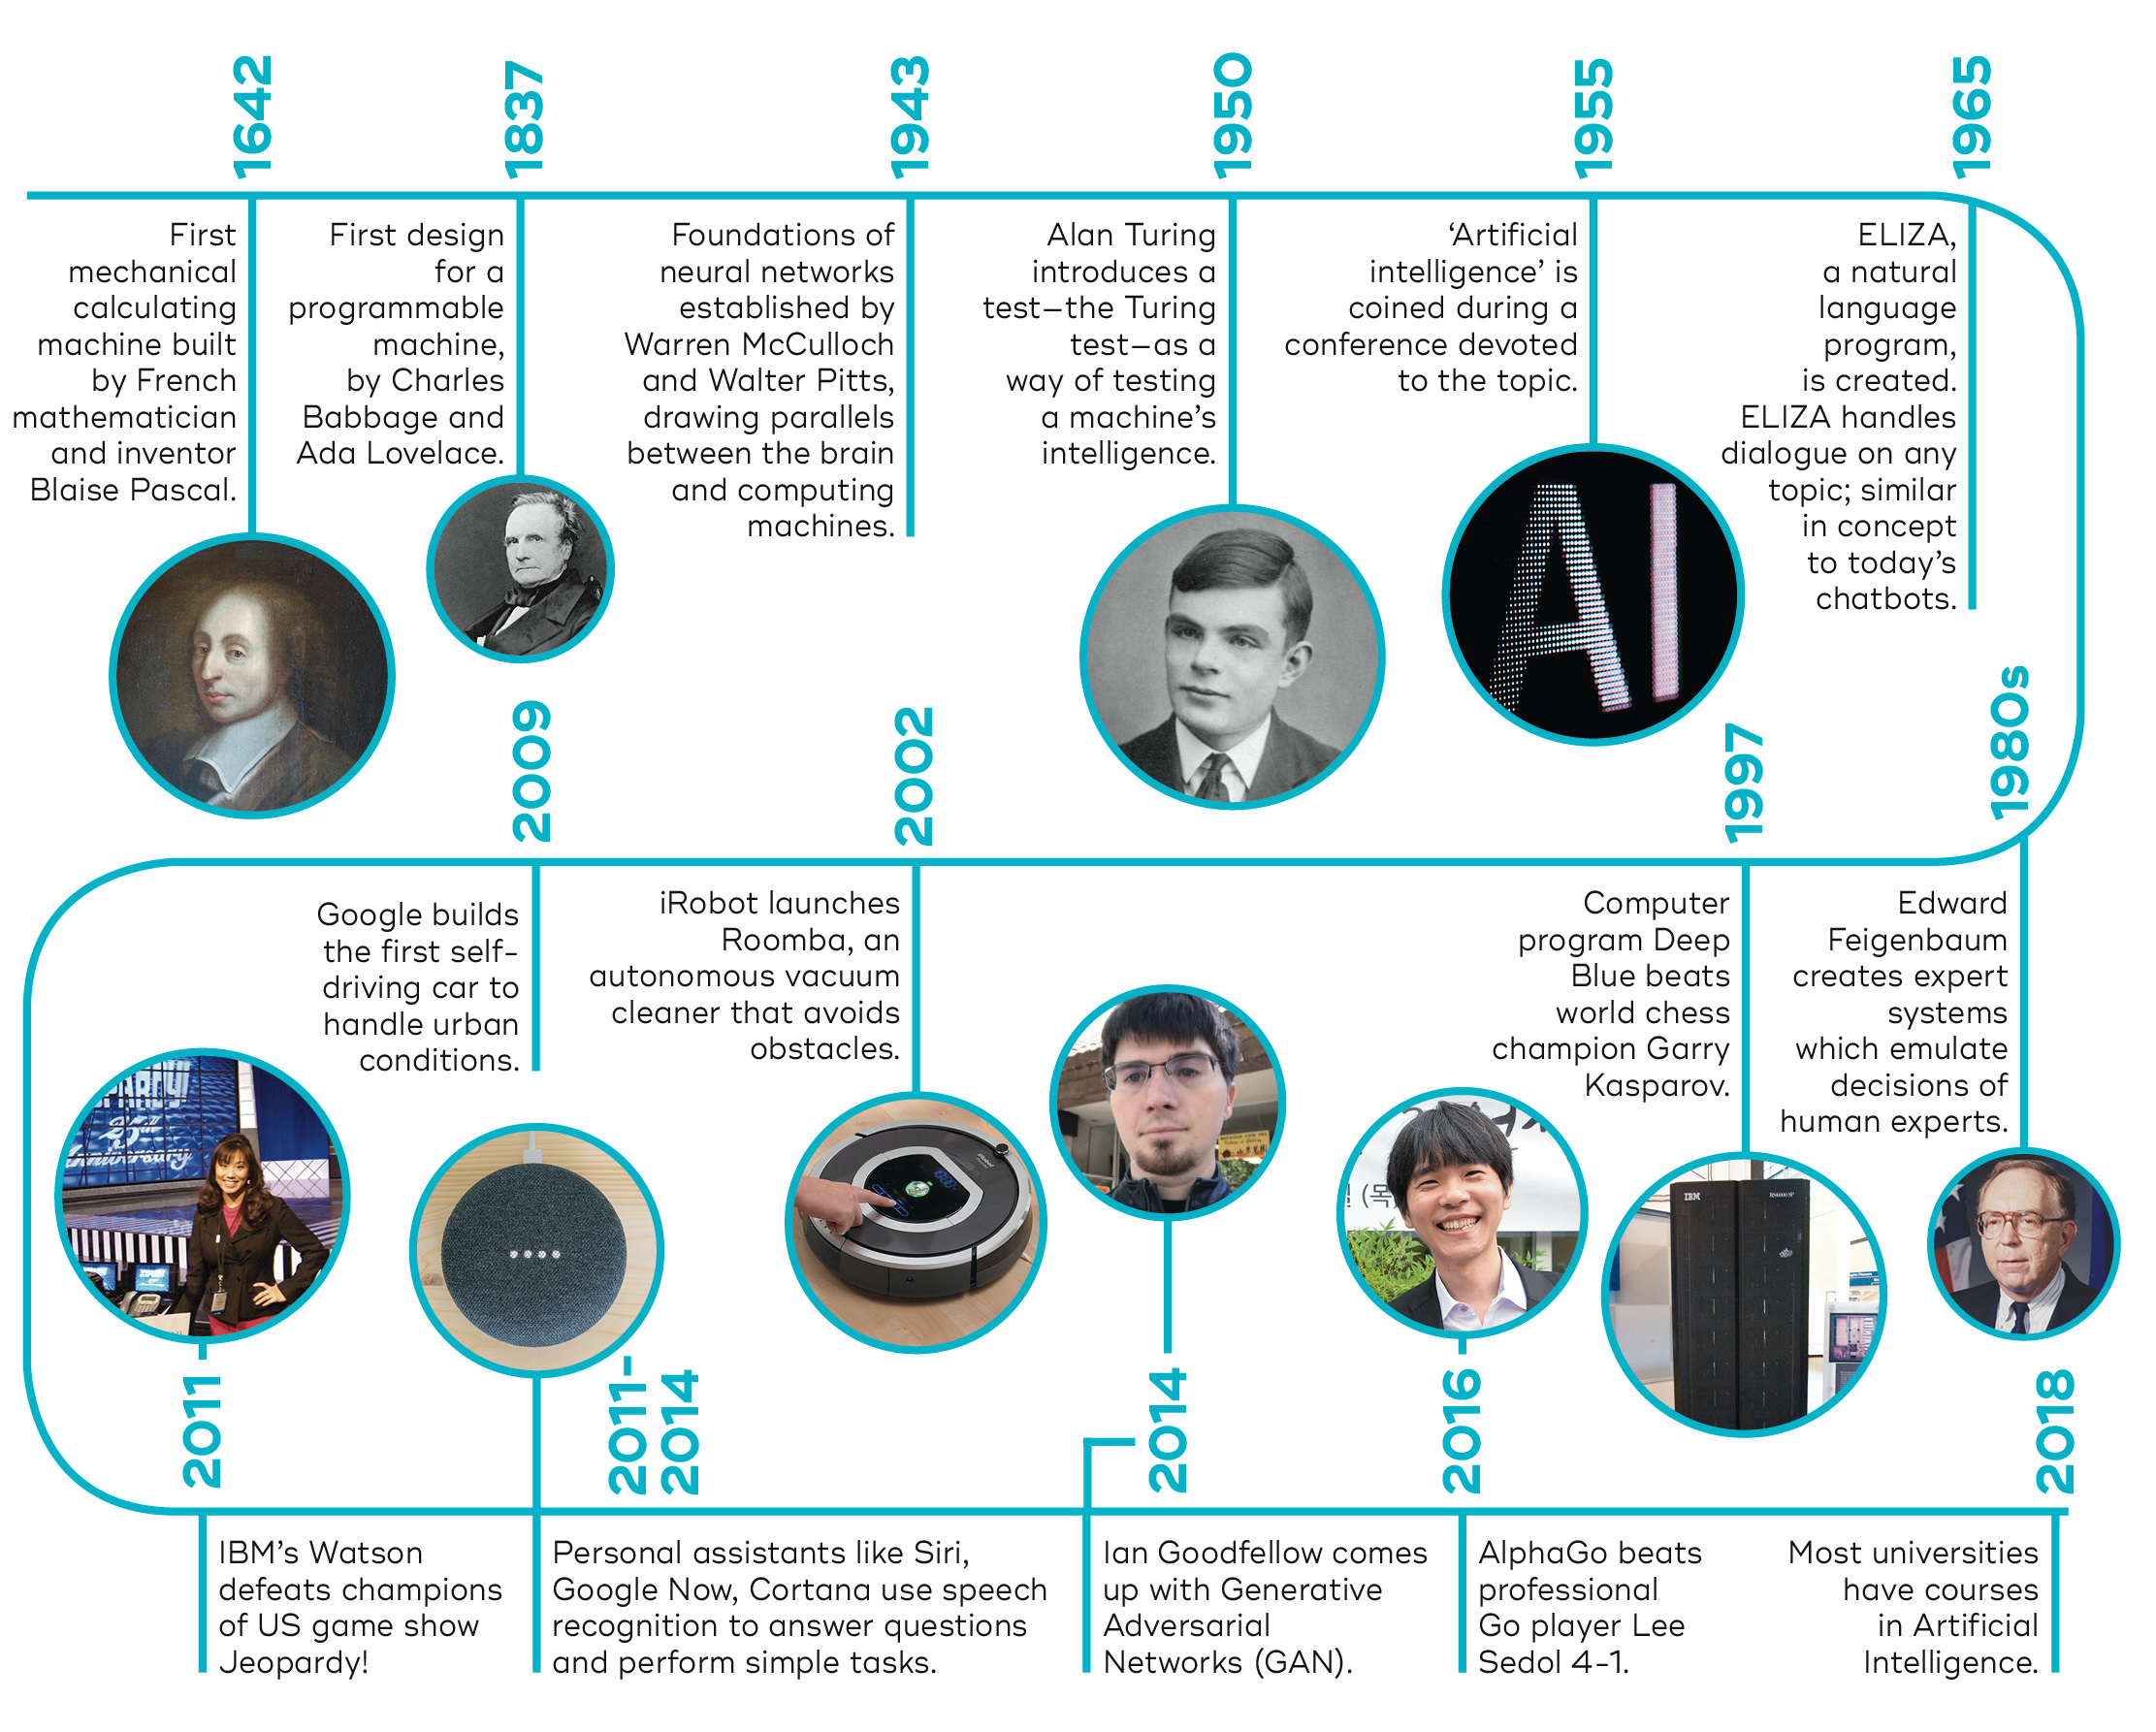
\includegraphics{ai-timeline.jpg}
        \caption{This diagram shows the development of the more cutting edge of AI tools proposed or deployed.}
        \label{fig:my_label}
\end{figure}

\newpage
\section{Intelligent Agents}

\subsection{What is an intelligent computational agent?}

\begin{itemize}
    \item An \textbf{agent} is something that \textbf{acts} in an environment. 
    \begin{itemize}
        \item Usually an agent has some autonomy, that is, it can follow it's own goals and it has it's own reasoning processes.
        \item An agent is quite different from an object in OOP, 
        \begin{itemize}
            \item For example, an object receives commands or requests, has internal processes that it executes and then returns values.
            \item Whereas the key difference between an agent and an object is that an agent has a sense of autonomy (that is, doing something for its own good). 
            \item So you can ask an agent to do something for you and it does not align with its goals or desires, it might not do what you requested for.
            \item Thus, the sense of autonomy is the defining feature that separates an agent (or agency) from an object.
            \item This difference is important because although agents will be developed using objects in python, they are not essentially objects because they will have a greater sense of autonomy and freedom to act and pursue their own goals. 
        \end{itemize}
    \end{itemize}
    \item An agent acts \textbf{intelligently} if...
    \begin{itemize}
        \item Its actions are appropriate for its goals and circumstances
        \begin{itemize}
            \item That is, at base level it is doing something sensible
        \end{itemize}
        \item It is flexible to changing environments and goals
        \begin{itemize}
            \item The idea that an agent can adapt to changing situations and different instructions.
        \end{itemize}
        \item It learns from experience
        \begin{itemize}
            \item It has a way of incorporating new knowledge and new information into its decision making 
        \end{itemize}
        \item It makes appropriate choices given perceptual and computational limitations.
        \begin{itemize}
            \item It can actually implement actions that achieve the goals it wants to attain. 
            \item Even if it has poor sensing capabilities and computational power. That is shortage of time and high computational hardware.
        \end{itemize}
    \end{itemize}
\end{itemize}


\subsection{Examples of agents}

\emph{Not necessarily computational agents}\\

\noindent Things like...

\begin{itemize}
    \item \textbf{Organisations:} Microsoft, Facebook, Government of Australia, UQ, ITEE,...
    \begin{itemize}
        \item These all have agency.
        \item They can act, learn, and reason.
        \item They do what achieves their ends and not necessarily what others tell them to.
    \end{itemize}
    \newpage
    \item \textbf{People:} teacher, doctor, stock trader, engineer, researcher, travel agent, farmer, waiter,...
    \begin{itemize}
        \item Any of these classes of occupations
        \item The people that are doing these jobs have agency. They choose what they do, they reason and they learn and thus try to achieve their goals.
    \end{itemize}
    \item \textbf{Computers and devices:} air-conditioner thermostat, airplane controller, network controller, movie recommendation system, tutoring system, diagnostic assistant, robot, GPS, navigation app, Mars rover...
    \begin{itemize}
        \item Some computers and devices, if they are appropriately setup can learn and reason from experience. \item They can adapt to change in situations and can be set for new different goals. 
    \end{itemize}
    \item \textbf{Animals:} dog, mouse, bird, insect, worm, bacterium, bacteria,...
    \begin{itemize}
        \item They can adapt to change in situations too, thus they have some agency as well.
        \item They evolve, which is a form of learning. 
    \end{itemize}
    \item book (?), sentence (?), word (?), letter (?)
    \begin{itemize}
        \item Can a book or article do things?
        \item Convince? Argue? Inspire? Cause people to act different? Learn from experience?
        \item These are not agents
    \end{itemize}
\end{itemize}

\newpage
\section{Goals of Artificial Intelligence}

\subsection{What are the goals of Artificial Intelligence?}

\begin{itemize}
    \item \textbf{Scientific Goal:} To understand the principles that make intelligent behavior possible in natural or artificial systems.
    \begin{itemize}
        \item So, essentially, what are the principles of intelligence that we can then use to engineer artificial intelligence or intelligent systems.
        \begin{itemize}
            \item Analyze natural and artificial agents.
            \item Formulate and test hypotheses about what it takes to construct intelligent agents
            \item Design, build, and experiment with computational systems that perform tasks that require intelligence
        \end{itemize}
    \end{itemize}
    \item \textbf{Engineering goal:} design useful, intelligent agents.
    \begin{itemize}
        \item Always make the "best" decision given the available resources (knowledge, time, computational power and memory)
        \begin{itemize}
            \item The catch here, is what does "best" entail?
            \begin{itemize}
                \item Is it maximizing the profit of the company you're working? (for example, Facebook) or are there ethical considerations that constrain what you should be doing?
                \item Thus, best is a difficult term to pin down but is quite fundamental to the way we design computational agents. 
            \end{itemize}
        \end{itemize}
        \item \textbf{Best:} Maximize certain performance measure(s), usually represented as a \textbf{\emph{utility function}}. 
        \begin{itemize}
            \item A utility function is a just a way of mapping outcomes to a score, effectively.
            \item In Economics, utility functions are usually associated with either actions that provide one with pleasure like eating a meal, going to see a movie, etc. weighted against the cost that you have to pay to do those things. The surplus you have here is your "utility". Its a construct, a way of thinking about things. But its really a way of mathmetising these sorts of problems so that we can use computational resources to solve them. 
            \item More on this throughout the semester, with increasing level of details.
        \end{itemize}
    \end{itemize}
\end{itemize}

\newline
\subsection{In this class...}

\begin{itemize}
    \item We are interested in building software systems (called agents) that behave rationally.
    \item i.e. Systems that accomplish what they are supposed to do, well, given the available resources.
    \begin{itemize}
        \item These resources can be information, computational, or time based. 
    \end{itemize}
    \item Don't worry about how close the systems resemble humans and about philosophical questions on what "intelligence" is (not that we are not interested in this!)
    \item But we may use inspirations from humans or other "intelligent" beings and systems.
\end{itemize}

\newpage
\section{Intelligent agents acting in an environment}

Here we will try to get more specific and precise about what we are trying to achieve through this course. 
\newline We are trying to define an intelligent that acts in an environment. Now this contains a few terms that we need to define concretely to be able to actually code in order to automate the reasoning, acting and learning in the decision making.
Now we will what we mean by \textbf{intelligent agents, acting, and an environment.}

\subsection{Recall our goal: To build a useful, intelligent agent}
To start with:
\begin{itemize}
    \item Computers perceive the world using sensors.
    \item Agents maintain models/representations of the world and use them for reasoning. 
    \item Computers can learn from data.
\end{itemize}

\noindent So, to achieve our goals, we need to define our \textbf{"agent"} in a way that we can \emph{program} it:
\begin{itemize}
    \item The problem of constructing an agent is usually called the \textbf{\emph{agent design problem.}}
    \begin{itemize}
        \item This design problem is the one that provides the agent sufficient autonomy to be flexible, adapt, learn, and reason. Effectively an engineering program.
    \end{itemize}
    \item Simply, it's about defining the components of the agent, so that when the agent acts rationally, it will accomplish the task it is supposed to perform, and do it well.
\end{itemize}

\noindent \textbf{\emph{Some important things we don't address in this course}}
\begin{itemize}
    \item \textbf{User Interaction:} Making the agents interact comfortable with humans is a substantial challenge for AI developers.
    \item \textbf{Ethics of AI:} AI applications can impact society in both positive and negative ways.
\end{itemize}


\newpage
\subsection{Agents acting in an environment: inputs and output}
An agent performs an action in the environment; the environment generates a percept or stimuli. The percept generated by the environment may depend on the sequence of actions the agent has done.

The term stimuli is often interchangeable with percept or feedback.

\begin{figure}[h!]
        \centering
        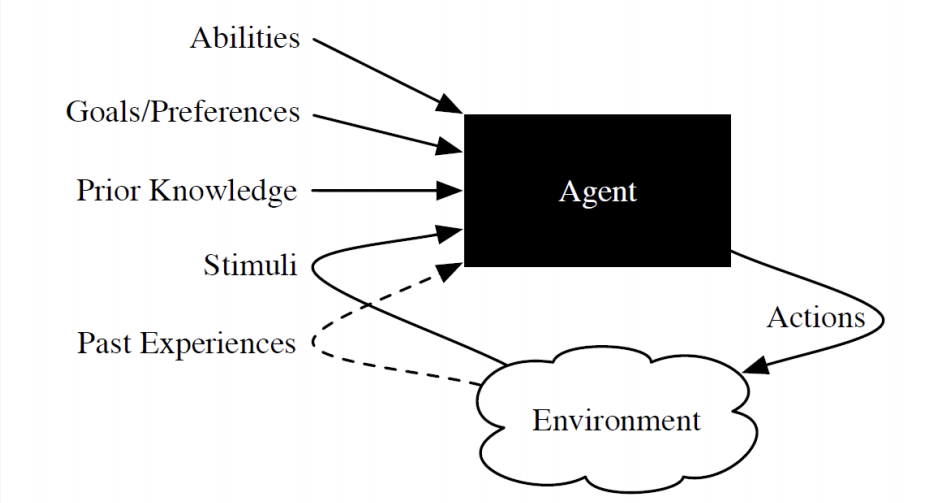
\includegraphics[scale=0.5]{agent-inputs-output.png}
        \caption{An agent undertaking actions which are fed into the environment with outputs from the environment}
        \label{fig:my_label}
\end{figure}

\noindent In addition to the history/past experiences and stimuli, an agent is equipped with knowing what its abilities, goals/preferences and some prior knowledge about how its environment works or how the agent itself works.\\
All of these are fed into the agent and incorporated into its decision making process and then agent has the opportunity to act in the environment.\\
From the environment it receives feedback and it adjusts its reasoning or decision making in a way that results in adjusting its actions and repeating the loop.

\begin{itemize}
    \item \textbf{Abilities:} the set of possible actions it can perform
    \item \textbf{Goals/Preferences:} what it wants, its desires, its values
    \item \textbf{Prior Knowledge:} what it knows and believes initially, what it doesn't get from experience
    \item \textbf{History of stimuli:}
    \begin{itemize}
        \item (current) \textbf{stimuli:} what it receives from environment now (observations, percepts)
        \item \textbf{past experiences:} what it has received in the past
    \end{itemize}
\end{itemize}

\newpage
\subsection{Examples of agents}

\subsubsection{Autonomous car}
\begin{itemize}
    \item \textbf{abilities:} steer, accelerate, brake
    \item \textbf{goals:}  safety, get to destination, timeliness...
    \item \textbf{prior knowledge:} street maps, what signs mean, what to stop for...
    \item \textbf{stimuli:} vision, laser, GPS, voice commands...
    \item \textbf{past experiences:}  how braking and steering affects direction and speed...
\end{itemize}\\

\subsubsection{Air-conditioner thermostat and controller agent}
\begin{itemize}
    \item \textbf{abilities:}  turn air-conditioner on or of
    \item \textbf{goals:} conformable temperature, save energy, save money
    \item \textbf{prior knowledge:} 24 hour cycle, weekends
    \item \textbf{stimuli:} temperature, set temperature, who is home, outside temperature, rooftop PV generation...
    \item \textbf{past experiences:} when people come and go, who likes what temperature, building
thermal dynamics...
\end{itemize}

\newpage
\section{Dimensions of Complexity}

Here we start unpacking why some problems are much harder than others.

\subsection{Dimensions of complexity in an agent design (P\&M Ch 1.5)}

\begin{itemize}
    \item Research proceeds by making simplifying assumptions (to get a handle on the situation), and gradually reducing (removing) these assumptions so that your simple model moves more towards the real world while still being based on sound principles.
    \item Each simplifying assumption gives or represents a dimension of complexity. Moving from simpler dimensions to more complex characteristics to match the real world better.
    \begin{itemize}
        \item Multiple values in a dimension: from simple to complex
        \item Simplifying assumptions can be relaxed in various combinations
        \item This results in different classes of problems. (We will go through possibly ten different classes of problems in this course).
    \end{itemize}
    \item Much of the history of AI can be seen as starting from the simple and adding in complexity in some of these dimensions.
\end{itemize}

\subsection{From P \& M Ch 1.5}

\begin{figure}[h!]
        \centering
        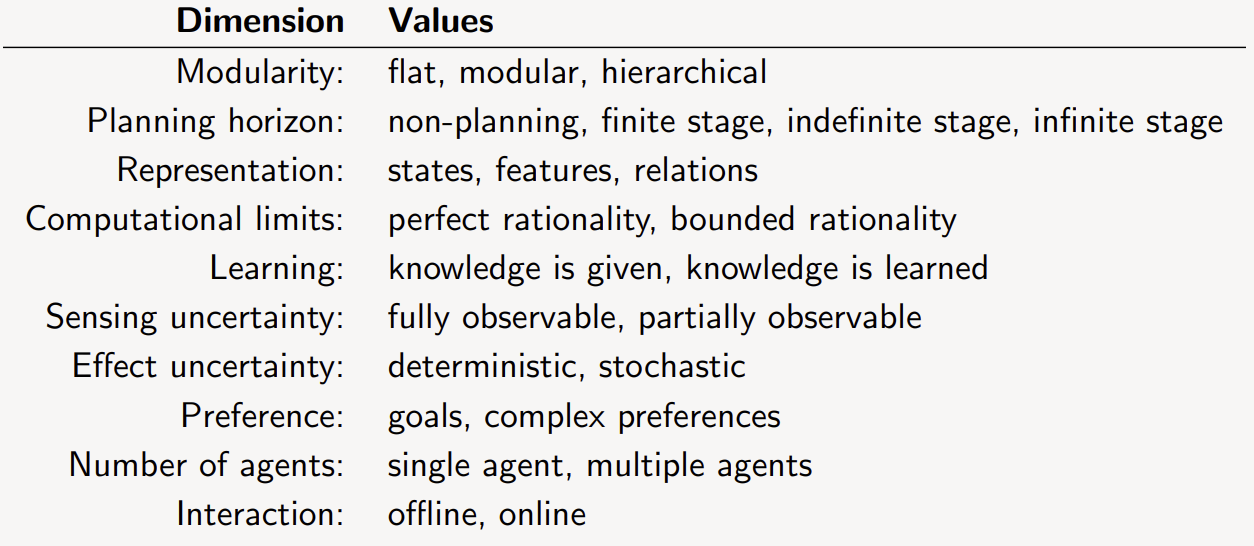
\includegraphics[scale=0.4]{definition-dimensions.png}
        \caption{Definitions of dimensions according to P\&M}
        \label{fig:my_label}
\end{figure}

\noindent The example of values and dimensions above in the figure not all-encompassing but are enough to provide an idea of the types of dimensions and the values they can take on.

\newpage
\subsection{Modularity}

By Modularity, we are talking about the structure of the overall big problem we're trying to solve.

\begin{itemize}
    \item Model at one level of abstraction: \textbf{flat}
    \begin{itemize}
        \item Typically the problems we're going to address in this course are going to be flat.
        \item That is, in the big problem there will only be a single sub problem
        \item But for more complex systems we have a hierarchy of problems.
    \end{itemize}
    \item Model with interacting modules that can be understood separately: \textbf{modular}
    \item Model with modules that are (recursively) decomposed into modules: \textbf{hierarchical}
    \item Flat representations are adequate for simple systems
    \item Complex biological systems, computer systems, organizations are all hierarchical.
\end{itemize}

\subsubsection{Is the environment continuous or discrete?}
\begin{itemize}
    \item A \emph{flat} description is typically either \textbf{continuous} (exclusive-or \textbf{discrete}.
    \item Hierarchical reasoning is often a hybrid of continuous and discrete
\end{itemize}

\subsection{Planning horizon}
...how far the agent looks into the future when deciding what to do.

\begin{itemize}
    \item \textbf{Static:} world does not change
    \item \textbf{Finite stage:} agent reasons about a fixed finite number of time steps
    \item \textbf{Indefinite stage:} agent reasons about a finite, but not predetermined, number of time
steps
    \item \textbf{Infinite stage:} the agent plans for going on forever (i.e. process oriented rather than an end goal as such.)
\end{itemize}

\subsection{Representation}
Much of modern AI is about finding compact representations and exploiting the compactness for computational gains.\\
\noindent Representation becomes a really key element to how you set up the problem that you're trying to address.

\noindent An agent can reason in terms of:

\begin{itemize}
    \item \textbf{Explicit states:} a state is one way the world could be
    \item \textbf{Features} or \textbf{Propositions.}
    \begin{itemize}
        \item States can be described using features.
        \item 30 binary features can represent 230 = 1, 073, 741, 824 states.
    \end{itemize}
    \item \textbf{Individuals} and \textbf{Relations}
    \begin{itemize}
        \items Are we dealing with an individual agent or are we dealing with relations {couldn't understand the word} between or are we dealing with abstract representations of agents that just comes across like an individual agent.  
        \item There is a feature for each relationship on each tuple of individuals.
        \item Often an agent can reason without knowing the individuals or when there are infinitely many
individuals.
    \end{itemize}
\end{itemize}

\subsection{Computational Limits}

\begin{itemize}
    \item \textbf{Perfect rationality:} the agent can determine the best course of action, without taking
into account its limited computational resources. That is, effectively no practical limit on the computation available to the agent.
    \item \textbf{Bounded rationality:} the agent must make good decisions based on its perceptual,
computational and memory limitations.
\end{itemize}

\subsection{Learning from Experience}
Whether the model is fully specified a priori:

\begin{itemize}
    \item \textbf{Knowledge is given.}
    \item \textbf{Knowledge is learned from data or past experience.}
\end{itemize}

\noindent In practice, there is always some mix of prior (innate, programmed) knowledge and learning (nature vs nurture). For example, The way you encode the mapping from percepts to learning routines is an example of prior knowledge being incorporated into the design of the agent. 

\subsection{Uncertainty}
We'll learn how to deal with uncertainty using probability and how we incorporate that into decision making at the start of module 3.\\
\noindent There are two dimensions for uncertainty:

\begin{itemize}
    \item \textbf{Sensing uncertainty} or noise perception
    \item \textbf{Effect uncertainty}
    \begin{itemize}
        \item Uncertainty about how your action affect the environment? 
    \end{itemize}
\end{itemize}\\

In this course, we restrict our focus to \textbf{probabilistic} models of uncertainty. Why?

\begin{itemize}
    \item Agents need to act even if they are uncertain.
    \item Predictions are needed to decide what to do:
    \begin{itemize}
        \item Definitive predictions: you will be run over tomorrow
        \item Point probabilities: probability you will be run over tomorrow is 0.002 if you are careful and
0.05 if you are not careful
        \item Probability ranges: you will be run over with probability in range [0.001,0.34]
    \end{itemize}
    \item Acting is gambling: agents who don’t use probabilities will lose to those who do.
    \item Probabilities can be learned from data and prior knowledge.
\end{itemize}

\subsection{Sensing uncertainty}
Whether an agent can determine the state from its stimuli:

\begin{itemize}
    \item \textbf{Fully-observable system:} the agent can observe perfectly the state of the world. We'll stick with this type of observable system for this course.    
    \item \textbf{Partially-observable:} there can be a number states that are possible given the agent’s
stimuli.
\end{itemize}

\subsection{Effect uncertainty}
If an agent knew the initial state and its action, could it predict the resulting state?\\

\noindent The dynamics can be:

\begin{itemize}
    \item \textbf{Deterministic:} the resulting state is determined from the action and the state
    \item \textbf{Stochastic:} there is uncertainty about the resulting state.
\end{itemize}

\subsection{Preferences}
What does the agent try to achieve?

\begin{itemize}
    \item \textbf{Achievement goal} is a goal to achieve. This can be a complex logical formula
    \item \textbf{Complex preferences} may involve trade-offs between various desiderata, perhaps at
different times.
    \begin{itemize}
        \item \textbf{Ordinal} only the order matters
        \item \textbf{Cardinal} absolute values also matter
    \end{itemize}
\end{itemize}

\noindent \textbf{Examples:} coffee delivery robot, medical doctor

\subsection{Number of agents}
Are there multiple reasoning agents that need to be taken into account?

\begin{itemize}
    \item \textbf{Single agent:} reasoning: any other agents are part of the environment.
    \item \textbf{Multiple agent:} reasoning: an agent reasons strategically about the reasoning of other
agents.
\end{itemize}

\noindent Agents can have their own goals: cooperative, competitive, or goals can be independent of
each other

\subsection{Interaction}
When does the agent reason to determine what to do?

\begin{itemize}
    \item \textbf{Reason offline:} before acting. For example, planning of the train schedule
    \item \textbf{Reason online:} while interacting with environment. For example, the roomba robot not knowing where the chairs are currently present in the room.
\end{itemize}

\newpage
\subsection{Dimensions of complexity in agent design}

\begin{figure}[h!]
        \centering
        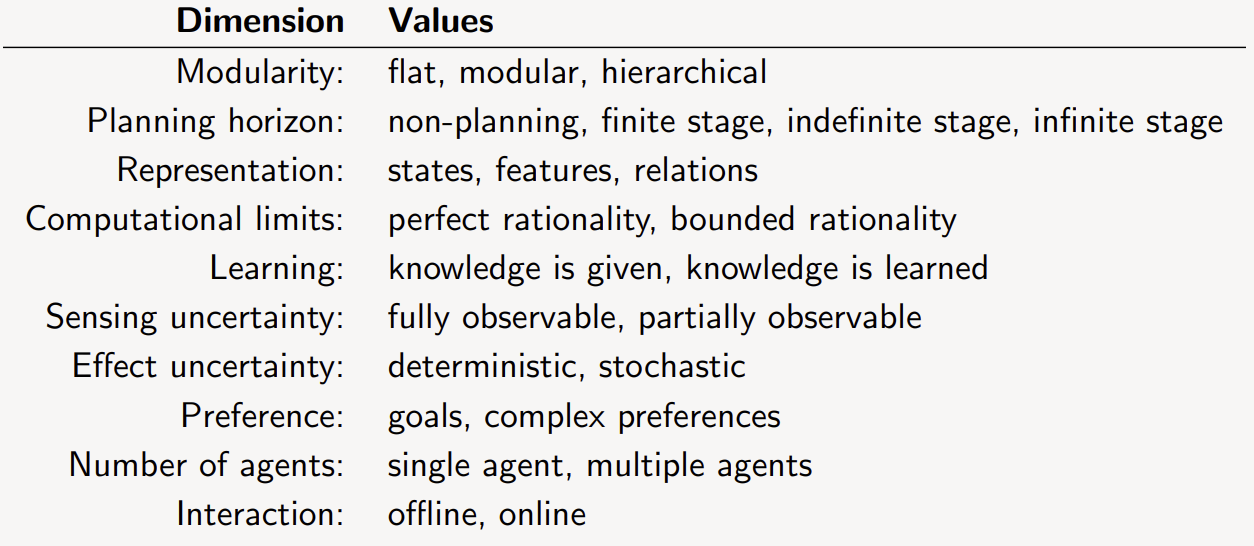
\includegraphics[scale=0.4]{definition-dimensions.png}
        \caption{Definitions of dimensions according to P\&M}
        \label{fig:my_label}
\end{figure}

\subsection{Example problem class: State-space search (Module 1)}

\begin{figure}[h!]
        \centering
        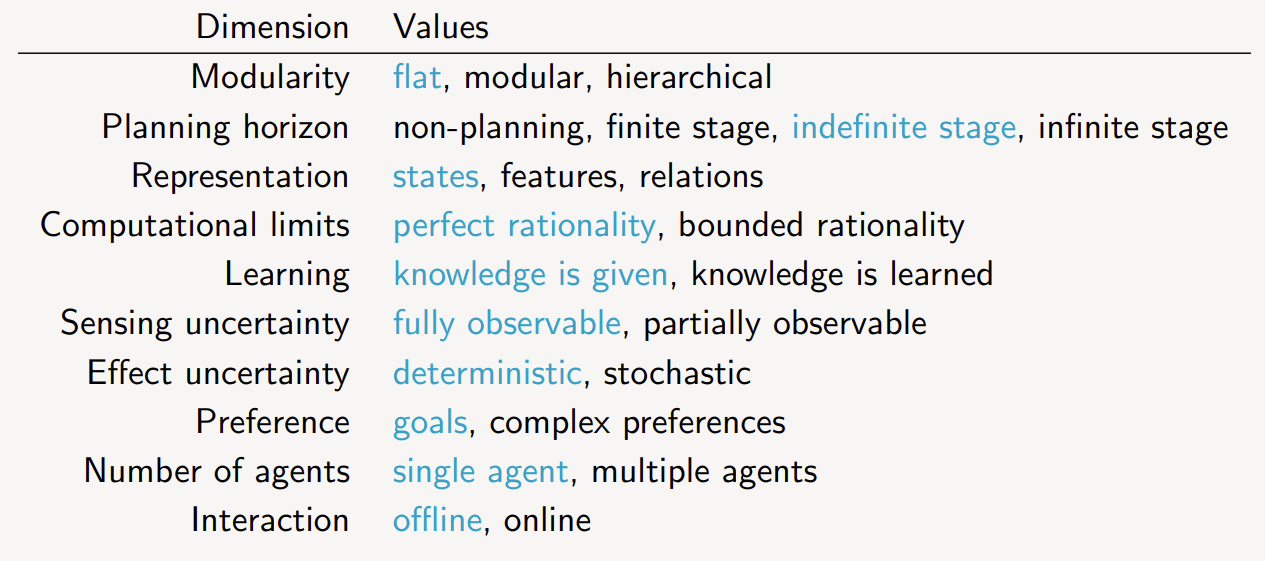
\includegraphics[scale=0.4]{module-1.png}
        \caption{}
        \label{fig:my_label}
\end{figure}

\newpage
\subsection{Example problem class: Deterministic planning using CSP (Module 2)}

\begin{figure}[h!]
        \centering
        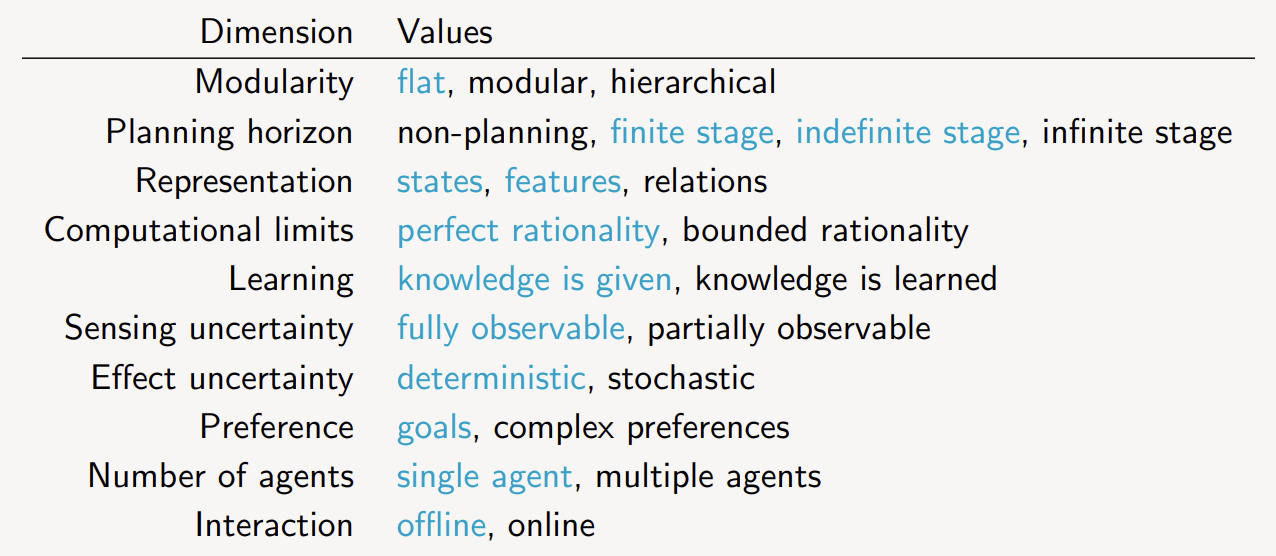
\includegraphics[scale=0.4]{module-2.png}
        \caption{}
        \label{fig:my_label}
\end{figure}

\subsection{Example problem class: Markov decision processes (MDPs, Module 3)}

\begin{figure}[h!]
        \centering
        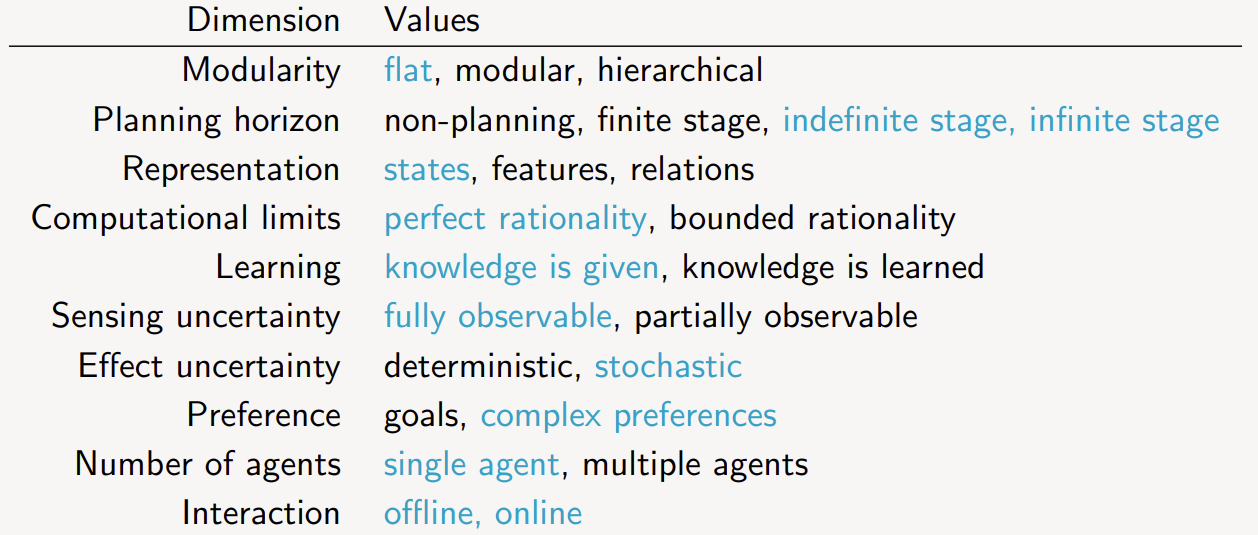
\includegraphics[scale=0.4]{module-3.png}
        \caption{}
        \label{fig:my_label}
\end{figure}

\newpage 
\subsection{Example problem class: Reinforcement learning (Module 4)}

\begin{figure}[h!]
        \centering
        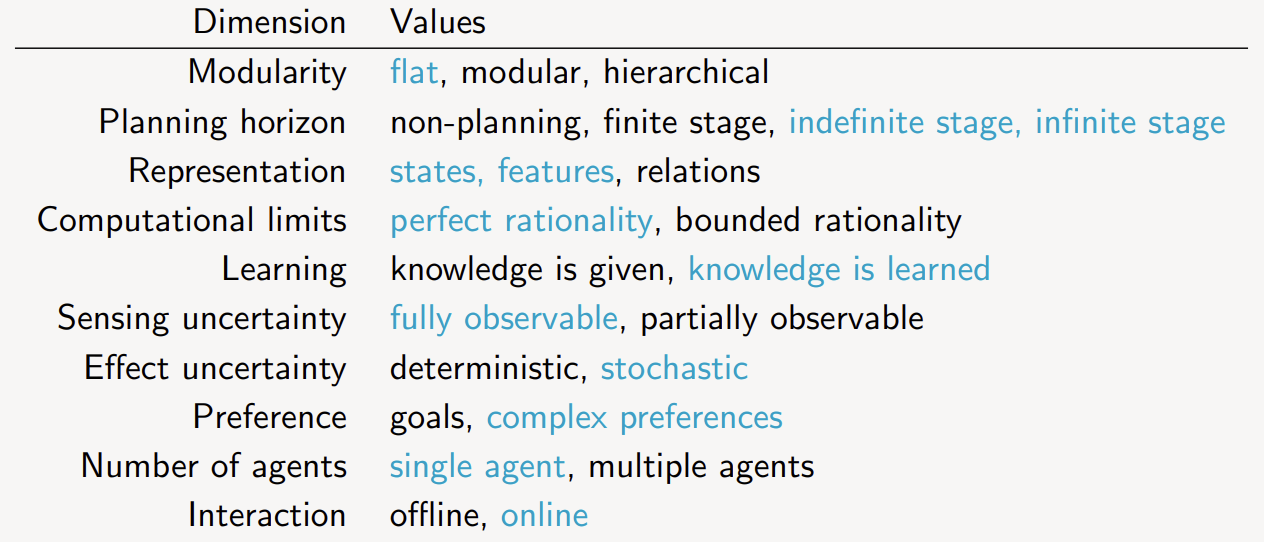
\includegraphics[scale=0.4]{module-4.png}
        \caption{}
        \label{fig:my_label}
\end{figure}

\subsection{Example problem class: Classical game theory (Module 5)}

\begin{figure}[h!]
        \centering
        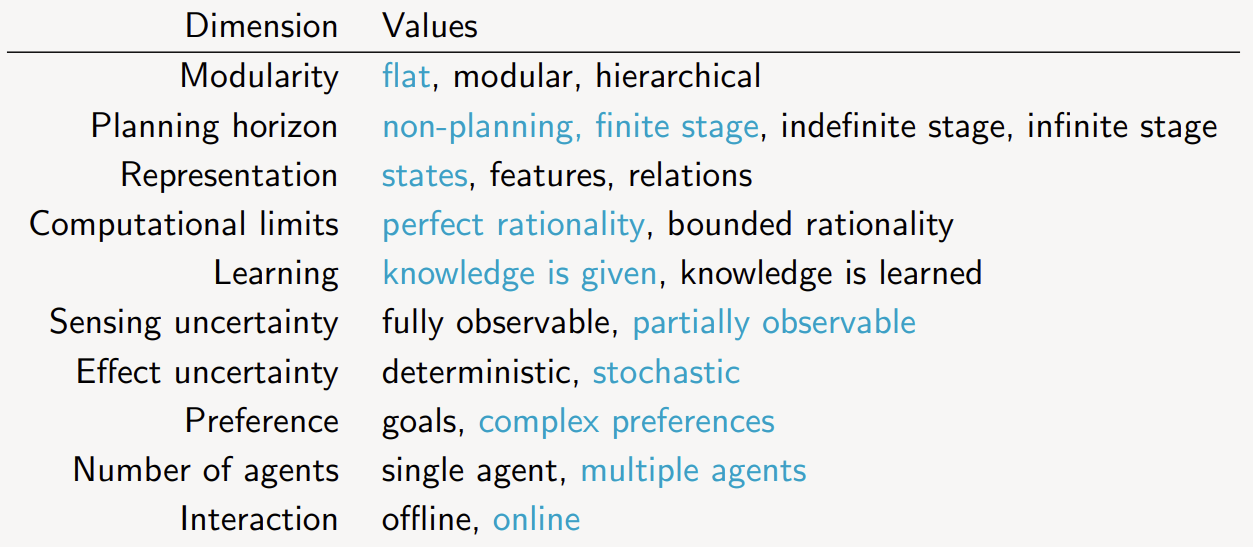
\includegraphics[scale=0.4]{module-5.png}
        \caption{}
        \label{fig:my_label}
\end{figure}

\newpage
\subsection{The real world: Humans}

\begin{figure}[h!]
        \centering
        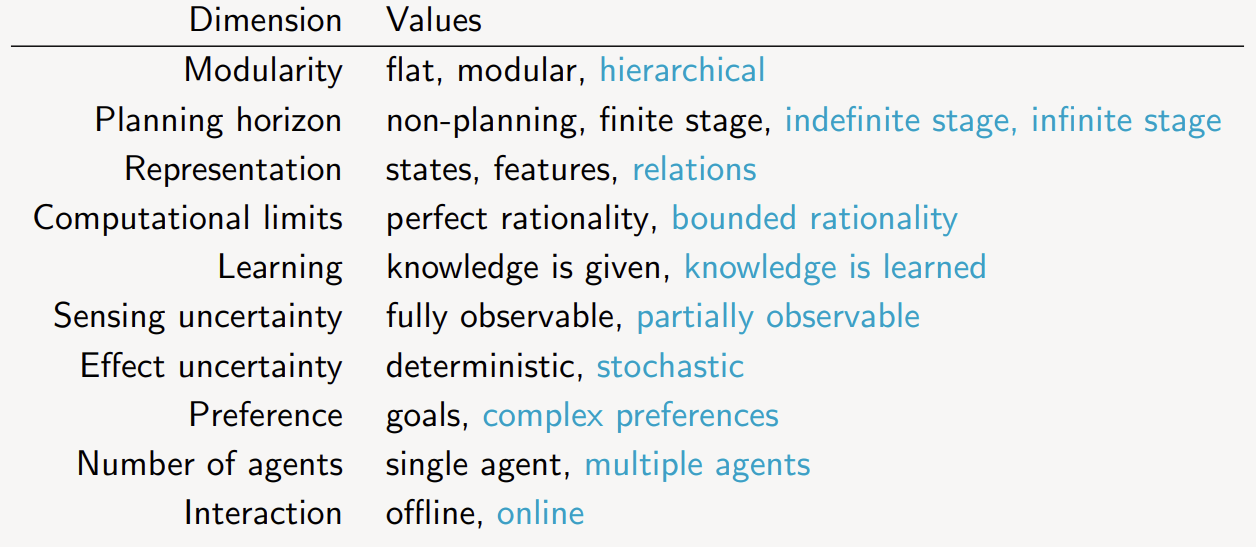
\includegraphics[scale=0.4]{human-dimensions.png}
        \caption{}
        \label{fig:my_label}
\end{figure}

\end{document}
